%Her gives en overordnet beskrivelse af systemets HW-design og SW-design. Den interne funktionalitet i de blokke/moduler/pakker/klasser, som blev beskrevet i afsnittet ”Arkitektur”, beskrives i en sådan grad at læseren efterfølgende kan forstå hvordan systemet er implementeret (bygget) HW-mæssigt og SW-mæssigt. HW-designet beskriver diagrammer (schematics) og beregning af komponentværdier. SW-designet beskriver særligt interessante/vanskelige dele af den interne logik i ”vanskelige” klasser/metoder, som er essentielle for at forstå deres funktionalitet. I projektrapporten skal HW/SW-designet beskrives på et overordnet plan. For yderligere detaljer angives reference til jeres ”designdokument” i projektets bilag.
\chapter{Design}

\section{Protocols}

This section describe the protocols used in the system. Communication between the the controller, server and client takes place using several .json files, JavaScript Object Notation. Communication between the GPS receiver, Navigation, and Autopilot modules in the controller uses the NMEA-0183 standard commonly used in marine navigation systems\cite{NMEA_wiki}. 

\subsection{Communication between server and client}

The system uses three .json files to send data between the controller, server, and client modules; fromNav.json, toNav.json, and activeParam.json. The latter contains the parameters the technician has specified for the system in the user interface, and an example can be seen in listing \ref{lst:activeParam}.

\begin{lstlisting}[caption = {Example of activeParam.JSON}, captionpos=b, label={lst:activeParam}, language=json,firstnumber=1]
{
	"name_": "Saint Princess",
	"parameter_names_": ["P", "I", "D", "Tool Width"],
	"parameters_": [10, 5, 1, 10],
	"creation_timestamp_": 1507201741743
}
\end{lstlisting}

This protocol could easily be extended to include more parameters that the technician could specify. A receiver class in the controller reads this file and sets the parameters in the autopilot.

Secondly, the toNav.json file contains the commands to the controller. An example is shown in listing \ref{lst:toNavBasic}

\begin{lstlisting}[caption = {Example of a calcP2P call in the toNav.JSON}, captionpos=b, label={lst:toNavCalcP2P}, language=json,firstnumber=1]
{
	"func_": "calcP2P",
	"target_position_": {
		"latitude_":56.187317092640775,
		"longitude_":10.18372267484665
	}
}
\end{lstlisting}

As seen, this command is to calculate a path to a certain coordinate given in latitude and longitude. 

The fromNav.json file contains all the user-relevant information for what's happening in the system. This includes the current path to traverse, how much of this path has already been completed, estimated time enroute (ETE), diagnostics data, such as connectivity data, motor status and telemetry, and timestamps in order to differentiate the file from previous versions.

 Examples of these components of the fromNav.json file, and more examples of the toNav.json and activeParam.json files, can be found in section~\ref{sec:protocols} on page~\pageref{sec:protocols} in the documentation.

\subsection{NMEA 0183 v2}

The NMEA standard is a naval standard developed by the National Marine Electronics Association. The protocol is comprised of ASCII characters, and are transferred over a serial connection. 

The messages used in the system are the GGA (GPS information) message from the GPS receiver to the navigation unit, an APB (Autopilot message with direction to steer, cross track error, and other information) message from the navigation to the autopilot, and a VTG (Vector Track and speed over the Ground) message also from the navigation to the autopilot. By using these standard messages, it is possible to remove a component from the system and insert a replacement that also follows this protocol, making the system much more modular.

The contents of these messages can be found in the documentation section~\ref{sec:protocols} on page~\pageref{sec:protocols}. 

\section{Hardware design}

Despite mainly being a software project, a considerable amount of hardware is required. The system requires a boat model, a controller unit, two motors, a battery, and a way to decouple the three modules from each other to avoid overcurrent and noise on the controller supply. 


\subsection{Boat}
The mechanical part of this project is the boat, "Saint Princess", as seen in figure~\ref{fig:saintprincess}. This boat was chosen simply because it was what was available, and since the project has been rather generic about the choice of hardware up to this point, it doesn't really matter. The boat has a motor in a so-called D-drive inboard configuration\cite{motor_config}, which means that the motor is inside the boat and is connected to the propeller via a shaft that goes out through the hull of the boat. The propeller sits just in front of the rudder, which is controlled by a servo on the inside. The hull of the boat is a deep vee hull\cite{hull-types}, it is a planning mode hull, which makes wakes smaller then other hull types.

\begin{figure}[H]
\centering
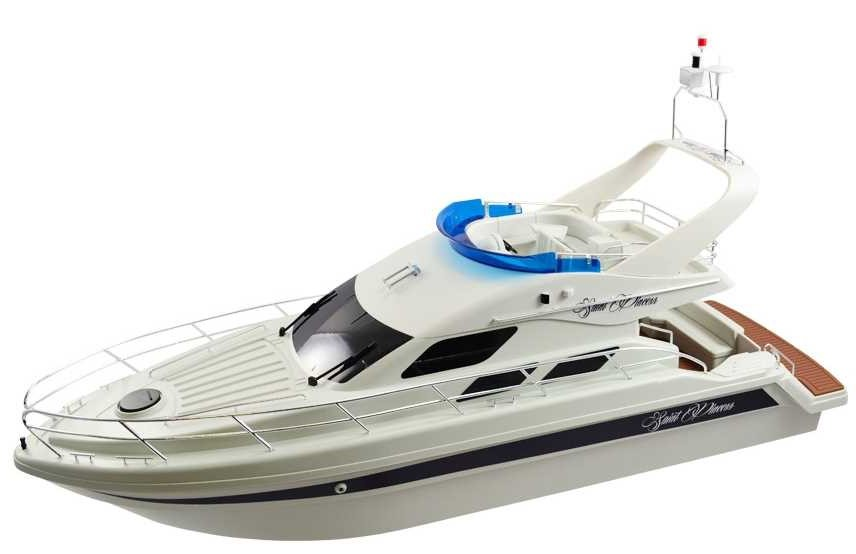
\includegraphics[width=0.5\linewidth]{saint_princess}
\caption{Saint Princess, a remote controlled yacht\cite{saint_princess}}
\label{fig:saintprincess}
\end{figure}

\subsection{System overview}

Figure ~\ref{fig:hardware_design} shows the overall hardware design. 

\begin{figure}[H]
\centering
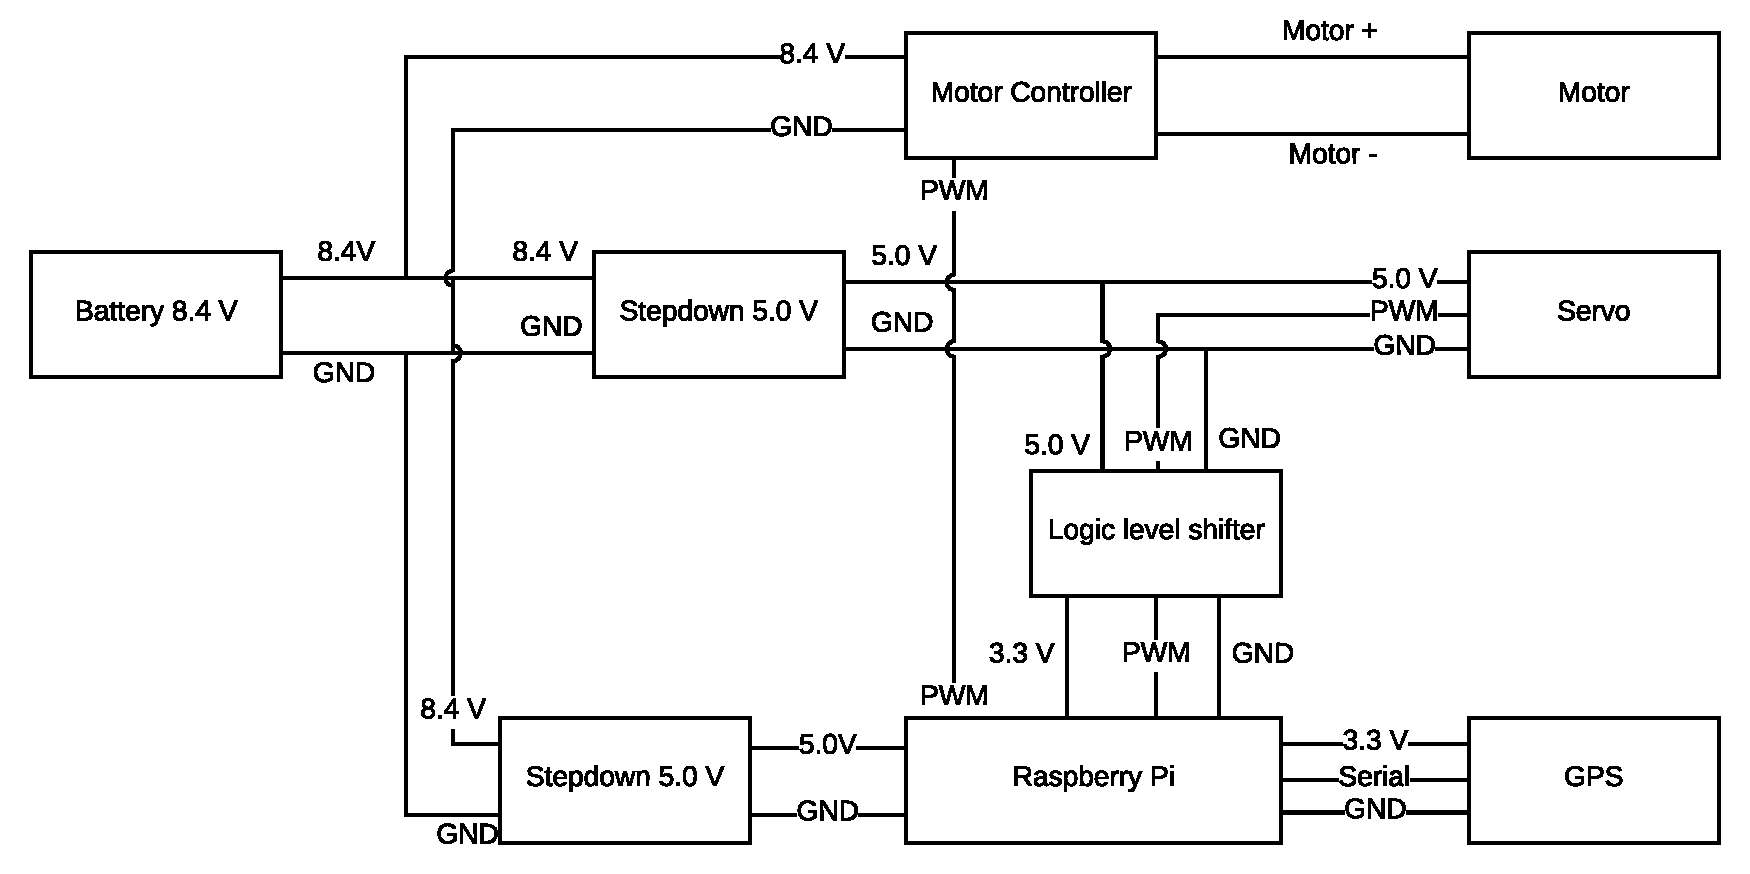
\includegraphics[width=1\linewidth]{Hardware_design}
\caption{Hardware design}
\label{fig:hardware_design}
\end{figure}

All components are supplied by a battery, which is stepped down for the controller and servo, and a logic level shifter is used between the controller and servo.

The controller chosen for the system is the Raspberry Pi model 3b, and the GPS receiver a Ublox Neo 7-M. The motor controller is a Cytron MD30C rev. 2, and the stepdown circuits used for the servo and controller are LM2596's which were available at the engineering school's Embedded Stock. The logic level shifter was likewise found in Embedded Stock.

A detailed explanation of why these components were chosen can be found in the hardware design section of the design, implementation, and test chapter in the documentation.

\section{Software design}
%TODO der skal ikke stå noge tom kode her
The project contains code in many different languages, totaling over 30000 lines. For brevity, this section only the design of the navigation and autopilot classes and their dependencies is included here. The full design can be seen in section~\ref{sec:software_design} on page~\pageref{sec:software_design} of the documentation.

Figure ~\ref{fig:Navigation} shows the overview of the navigation class and its dependencies. It is seen that the navigation uses a number of helper classes.

Coordinate which contains a latitude and longitude, CoverageRectangle which contains two Coordinates which define a rectangle on the map, TargetPosition containing one Coordinate, an enumerator containing the names of the commands the navigation module can execute.

NavigationData contains information about the path to complete, the estimated time enroute, and how much of the path has already been traversed. Pose contains a Coordinate for the current position, and an orientation. 

Along with the helper classes, Navigation has references to several interfaces: The Autopilot, GPS receiver, Receiver, and Transmitter interfaces. The Navigation module's own interface is seen at the top of the figure.

\begin{figure}[H]
\centering
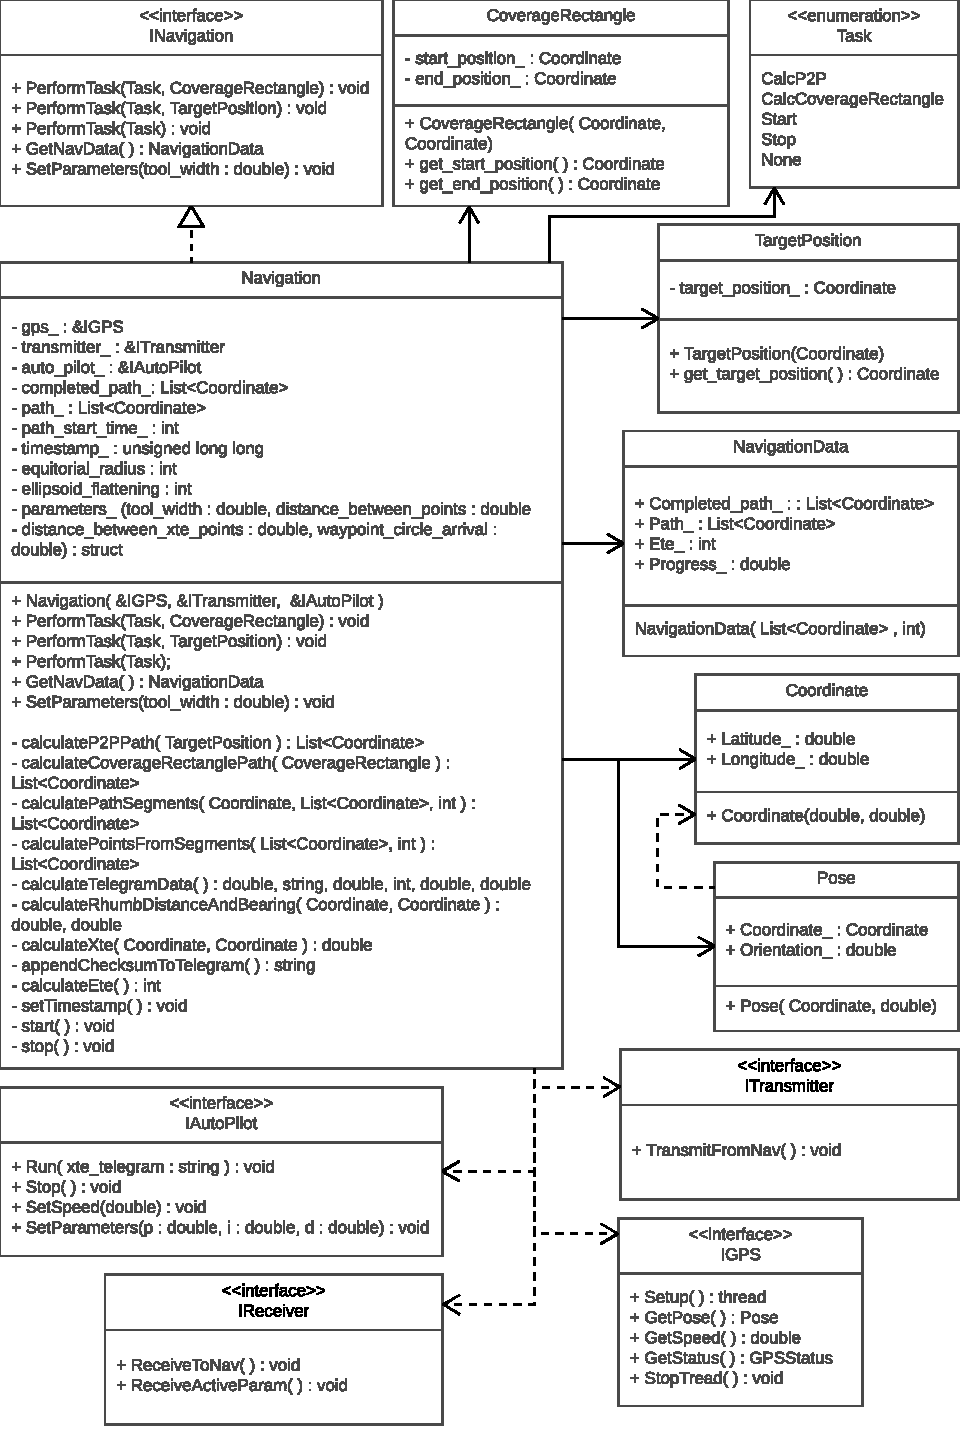
\includegraphics[max width=1\linewidth]{Navigation_class_diagram}
\caption{Navigation class diagram}
\label{fig:Navigation}
\end{figure}

Figure ~\ref{fig:Autopilot} shows the overview of the autopilot class and its dependencies. This module has an interface for the Navigation and Receiver to access, and has references to two interfaces; a position motor and a speed motor. 

\begin{figure}[H]
\centering
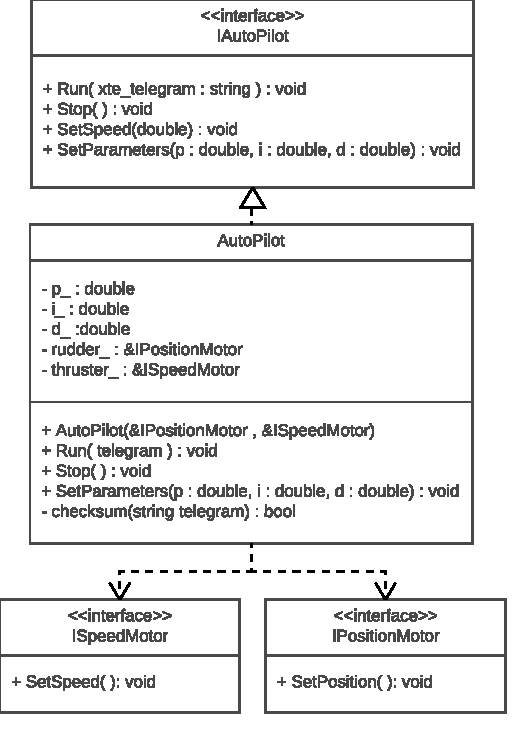
\includegraphics[max width=1\linewidth]{Autopilot_class_diagram}
\caption{Autopilot class diagram}
\label{fig:Autopilot}
\end{figure}